% !TEX program = xelatex
% !TeX spellcheck = en_GB-oed
\documentclass[10pt,a4paper,parskip=half,numbers=endperiod,parskip]{scrartcl}

%!TEX root = formalization.ftl.tex

\usepackage{comment}
\usepackage{tkz-euclide}
\usepackage[hidelinks]{hyperref}

\usepackage{auxhook} % Fixes auxhook (seems to be broken by etoolbox in naproche.sty)


\usepackage{amsmath}
\usepackage{amsthm}
\usepackage{thmtools}
%\usepackage{fontspec}


%\usepackage{newpxtext,newpxmath}

% Proza
%\setsansfont{ProzaLibre}[
%  Extension={.ttf},
%  Path=./fonts/proza/,
%  Scale=MatchLowercase,
%  UprightFont={*-Regular},
%  BoldFont={*-SemiBold},
%  ItalicFont={*-Italic},
%  BoldItalicFont={*-SemiBoldItalic}]

\RequirePackage{etoolbox}



% Sectioning
\addtokomafont{section}{\normalsize}
\RedeclareSectionCommand[
  runin=false,
  afterindent=false,
  beforeskip=0.5\baselineskip,
  afterskip=-0.5\baselineskip]{section}

\addtokomafont{subsection}{\normalsize}
\RedeclareSectionCommand[
    runin=true,
    afterindent=false,
    beforeskip=0pt,
    afterskip=0\baselineskip]{subsection}

\addtokomafont{pagenumber}{\sffamily}


% Main title and abstract

\addtokomafont{title}{\large}
\addtokomafont{author}{\normalsize}
\addtokomafont{date}{\normalsize}

\makeatletter
\renewcommand*{\@maketitle}{%
  \global\@topnum=\z@
  \setparsizes{\z@}{\z@}{\z@\@plus 1fil}\par@updaterelative
  \ifx\@titlehead\@empty \else
    \begin{minipage}[t]{\textwidth}
      \usekomafont{titlehead}{\@titlehead\par}%
    \end{minipage}\par
  \fi
  \null
  \vskip 2em%
%  \begin{center}%
    \ifx\@subject\@empty \else
      {\usekomafont{subject}{\@subject \par}}%
      \vskip 1.5em
    \fi
    {\usekomafont{title}{\@title \par}}%
    \vskip .5em
    {\ifx\@subtitle\@empty\else\usekomafont{subtitle}\@subtitle\par\fi}%
    \vskip 1em
    {%
      \usekomafont{author}{%
        \lineskip .5em%
        \begin{tabular}[t]{@{}l}
          \@author
        \end{tabular}\par
      }%
    }%
    \vskip 1em%
    {\usekomafont{date}{\@date \par}}%
    \vskip \z@ \@plus 1em
    {\usekomafont{publishers}{\@publishers \par}}%
    \ifx\@dedication\@empty \else
      \vskip 2em
      {\usekomafont{dedication}{\@dedication \par}}%
    \fi
%  \end{center}%
  \par
  \vskip 2em
}%

\renewenvironment{abstract}{%
  \if@titlepage
    \titlepage
    \null\vfil
    \@beginparpenalty\@lowpenalty
    \if@abstrt
      \begin{center}
        \normalfont\sectfont\nobreak\abstractname
        \@endparpenalty\@M
      \end{center}
    \fi
  \else
    \section*{Abstract}
    \if@twocolumn\if@abstrt
        \addsec*{\abstractname}
      \fi
    \else
      \if@abstrt
        \small
        \begin{flushleft}
          {\normalfont\sectfont\nobreak\abstractname
            \vspace{-.5em}\vspace{\z@}}%
        \end{flushleft}
      \fi
%      \quotation
    \fi
  \fi
}{%
  \if@titlepage
    \par\vfil\null\endtitlepage
  \else
    \if@twocolumn\else
%       \endquotation
            \par
    \fi
  \fi
}
\makeatother



%% Space between paragraphs in proofs in ForTheL environments
\newlength{\ftlparskip}
\setlength{\ftlparskip}{1em}

\newenvironment{forthel}{%
  \setbool{forthel}{true}%
}{%
  \setbool{forthel}{false}%
}

\newtheoremstyle{formalized}% name of the style to be used
    {-0.5\baselineskip}% measure of space to leave above the theorem. E.g.: 3pt
    {-0.5\baselineskip}% measure of space to leave below the theorem. E.g.: 3pt
    {\normalfont} % name of font to use in the body of the theorem
    {0pt}% measure of space to indent
    %{\sffamily\itshape}% name of head font
    {\sffamily\bfseries}% name of head font
    {}% punctuation between head and body
    { }% space after theorem head; " " = normal inter-word space
    %{\thmname{#1}\thmnumber{ #2}. \thmnote{ (#3) }}
    {{\upshape\thmnumber{#2}.} \thmname{#1}\thmnote{ (#3)}. }


\theoremstyle{formalized}


% Theorem environments without numbering.
\newtheorem*{quotedaxiom}{Axiom}
\newtheorem*{quotedcorollary}{Corollary}
\newtheorem*{quoteddefinition}{Definition}
\newtheorem*{quotedfact}{Fact}
\newtheorem*{quotedlemma}{Lemma}
\newtheorem*{quotedproposition}{Proposition}
\newtheorem*{quotedremark}{Remark}
\newtheorem*{quotedsignature}{Signature}
\newtheorem*{quotedtheorem}{Theorem}



\declaretheoremstyle[
  headfont={},
  headformat={\bfseries\sffamily\NUMBER.} {\mdseries\rmfamily\itshape\NAME}\NOTE,
  numbered=yes,
  bodyfont=\normalfont,
  spaceabove=-0.5\baselineskip plus 0.05em minus 0.05em,
  %prefoothook={\hfill{}---},
  %prefoothook={\ ---},
  spacebelow=-0.5\baselineskip plus 0.05em minus 0.05em,
]{newformalized}


\declaretheorem[numberwithin=section,style=newformalized,Axiom,refname={axiom,axioms},Refname={Axiom,Axioms}]{axiom}
\declaretheorem[numberlike=axiom,style=newformalized,Signature,refname={signature,signatures},Refname={Signature,Signatures}]{signature}
\declaretheorem[numberlike=axiom,style=newformalized,Convention,refname={convention,conventions},Refname={Convention,Conventions}]{convention}
\declaretheorem[numberlike=axiom,style=newformalized,Theorem,refname={theorem,theorems},Refname={Theorem,Theorems}]{theorem}
\declaretheorem[numberlike=axiom,style=newformalized,Definition,refname={definintion,definitions},Refname={Definition,Definitions}]{definition}
\declaretheorem[numberlike=axiom,style=newformalized,Lemma,refname={lemma,lemmas},Refname={Lemma,Lemmas}]{lemma}


% More visible line breaks in proofs.
% ===================================

\newbool{forthel}

\let\originalproof\proof
\let\originalendproof\endproof

% Set length of \parskip to \ftlparskip in proofs in ForTheL environments.
%
% NOTE: "\vspace*{-\parskip}" is necessary to avoid additional space between
% theorem and proof
\renewenvironment{proof}{%
  \originalproof%
  \ifbool{forthel}{\setlength{\parskip}{\ftlparskip}\vspace*{-\parskip}}%
  \relax%
}
{%
  \originalendproof%
}


% Symbols
% =======

\newcommand{\Cong}[4]{#1 #2 \equiv #3 #4}
\newcommand{\NotCong}[4]{#1 #2 \not\equiv #3 #4}
\newcommand{\Betw}[3]{#1 #2 #3}
\newcommand{\Col}[3]{\operatorname{Col}(#1, #2, #3)}
\newcommand{\SenaryCong}[6]{#1 #2 #3 \equiv #4 #5 #6}
\newcommand{\BetwFour}[4]{#1 #2 #3 #4}
\newcommand{\BetwFive}[5]{#1 #2 #3 #4 #5}
\newcommand{\BetwSix}[6]{#1 #2 #3 #4 #5 #6}
\newcommand{\Leq}[4]{#1 #2 \leq #3 #4}
\newcommand{\Geq}[4]{#1 #2 \geq #3 #4}
\newcommand{\Less}[4]{#1 #2 < #3 #4}
\newcommand{\Greater}[4]{#1 #2 > #3 #4}
\newcommand{\RelEquiv}[3]{#1 \approx_{#3} #2}

\newcommand{\Ray}[2]{\operatorname{Ray}(#1 #2)}

\newcommand{\OFS}[8]{\operatorname{OFS}%
\left(
\begin{smallmatrix}%
#1 & #2 & #3 & #4 \\
#5 & #6 & #7 & #8
\end{smallmatrix}%
\right)%
}
\newcommand{\IFS}[8]{\operatorname{IFS}
\left(
\begin{smallmatrix}%
#1 & #2 & #3 & #4 \\
#5 & #6 & #7 & #8
\end{smallmatrix}
\right)%
}
\newcommand{\FS}[8]{\operatorname{FS}
\left(
  \begin{smallmatrix}%
#1 & #2 & #3 & #4 \\
#5 & #6 & #7 & #8
\end{smallmatrix}
\right)%
}


\title{Beginnings of Tarskian geometry in Naproche}
\author{Adrian De Lon (2019--2021), Daniel Nogues Kollert (2019)}
\date{2021-02-13}

\usepackage[british]{babel}
\usepackage{comment}


\begin{document}
  %\maketitle
  \begin{flushleft}
    Adrian De Lon (2019--2021), Daniel Nogues Kollert (2019)
    \\ University of Bonn
    \\ 13th February 2021
    \\ This note is licensed under a {CC0 1.0} license.
  \end{flushleft}

  \vspace*{2\baselineskip}

  {\large\bfseries\sffamily Beginnings of Tarskian geometry in Naproche (draft)}


  \begin{abstract}
    We present a %self-contained
    literate formalization of the beginnings of Tarskian geometry.
    We follow
    \textit{Metamathematische Methoden in der Geometrie}
    by Schwabhäuser, Szmielew, and Tarski ({SST}),
    covering most of the material up to Satz 6.7\kern-1pt,
including Gupta's result that outer Pasch follows from inner Pasch.
    Throughout, figures help the human reader keep up with the automated theorem prover.
  \end{abstract}

  \section{Introduction}

  Tarski's axiomatization of geometry is characterized by its logical elegance, relying only on two basic relations between points
  and a few simple axioms.
  These properties make Tarskian geometry attractive for formalization:
  in particular for research in automated deduction, see for instance Narboux (2006), Beeson and Wos (2017).
  For more detailed accounts of Tarski's axioms and their history see
  {SST}, Beeson (2015), and Narboux (2006).

  \section{The language of Tarskian geometry}

  The only objects under consideration are \textit{points}.
  They are subject to two primitive relations:
  quaternary \textit{congruence} ${(-)}{(-)}{\equiv}{(-)}{(-)}$
  and ternary \textit{betweenness} $\Betw{(-)}{(-)}{(-)}$.
  Congruence (also called \textit{equidistance}) expresses that the distance between the first two points is equal to the distance of the last two points, and betweenness expresses that
  the second point lies between the other two on a shared line.
  Informally we will also talk about segments and lines,
  indicating them by concatenation $(-)(-)$ of points.

\begin{comment}
  \begin{forthel}
    [synonym point/-s]
  \end{forthel}
\end{comment}

  \begin{forthel}
    \begin{signature}
      A point is an object.
    \end{signature}
  \end{forthel}

  \begin{convention}
    \begin{forthel}
      Let $a, b, c, d, e, f$ denote points.
    \end{forthel}
  \end{convention}

  \begin{forthel}
    \begin{signature}[Congruence]
      $\Cong{a}{b}{c}{d}$ is a relation.
    \end{signature}
  \end{forthel}

  \begin{convention}
    \begin{forthel}
      %Let $x$ and $y$ are congruent to $v$ and $w$ stand for $\Cong{x}{y}{v}{w}$.
      %Let $\NotCong{x}{y}{v}{w}$ stand for $x$ and $y$ are not congruent to $v$ and $w$.
      Let $\NotCong{a}{b}{c}{d}$ stand for it is wrong that $\Cong{a}{b}{c}{d}$.
    \end{forthel}
  \end{convention}

  \begin{forthel}
    \begin{signature}[Betweenness]
      $\Betw{a}{b}{c}$ is a relation.
    \end{signature}
  \end{forthel}

  Points are \textit{collinear} when they lie on a single line.
  We will later see that betweenness is symmetric
  ($\Betw{a}{b}{c}$ implies $\Betw{c}{b}{a}$),
  so we only need to consider three of the six permutations of three points in the definition of collinearity.

  \begin{forthel}
    \begin{definition}[Collinearity]
      $a$ is collinear with $b$ and $c$ iff $\Betw{a}{b}{c}$ or $\Betw{b}{c}{a}$ or $\Betw{c}{a}{b}$.
    \end{definition}
  \end{forthel}




  \begin{forthel}
    \begin{axiom}[Reflexivity of congruence] % SST A1
      We have $\Cong{a}{b}{b}{a}$.
    \end{axiom}
  \end{forthel}


  \begin{forthel}
    \begin{axiom}[Pseudotransitivity of congruence] % SST A2
      If $\Cong{c}{d}{a}{b}$ and $\Cong{c}{d}{e}{f}$ then $\Cong{a}{b}{e}{f}$.
    \end{axiom}
  \end{forthel}


  \begin{forthel}
    \begin{axiom}[Identity of congruence] % SST A3
      If $\Cong{a}{b}{c}{c}$ then $a = b$.
    \end{axiom}
  \end{forthel}


  Segment construction allows us to extend a segment $ab$
  by a length specified by another segment $de$.

  \begin{forthel}
    \begin{axiom}[Segment construction]\label{segment_construction} % SST A4
      There exists a point $c$ such that $\Betw{a}{b}{c}$ and $\Cong{b}{c}{d}{e}$.
    \end{axiom}
  \end{forthel}


  We say that the points $x,y,z,r,u,v,w,p$ are in an
  \textit{outer five segment configuration}
  whenever $\OFS{x}{y}{z}{r}{u}{v}{w}{p}$.

  \begin{convention}
    \begin{forthel}
        Let $a', b', c', d'$ denote points.
        Let $x, y, z, u, v, w, p, q, r$ denote points.
      \end{forthel}
  \end{convention}

  %This is definition 2.10 in \textit{SST}.
  \begin{forthel}
    \begin{definition}
      $\OFS{x}{y}{z}{r}{u}{v}{w}{p}$ if and only if
      $\Betw{x}{y}{z}
        \wedge \Betw{u}{v}{w}$
      and we have
      $\Cong{x}{y}{u}{v}
        \wedge \Cong{y}{z}{v}{w}
        \wedge \Cong{x}{r}{u}{p}
        \wedge \Cong{y}{r}{v}{p}$.
    \end{definition}
  \end{forthel}

  Using the concept of an outer five segment configuration,
  we can state the five segment axiom in a concise form.

  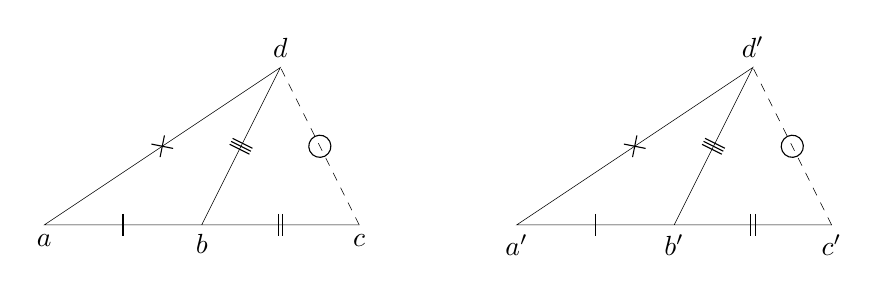
\begin{tikzpicture}
    % Points
    \tkzDefPoint (0,0){a}
    \tkzDefPoint (2,0){b}
    \tkzDefPoint (4,0){c}
    \tkzDefPoint (3,2){d}
    \tkzDefPoint (6,0){a'}
    \tkzDefPoint (8,0){b'}
    \tkzDefPoint (10,0){c'}
    \tkzDefPoint (9,2){d'}
    % Segments
    \tkzDrawPolySeg (b,a,d,b,c)
    \tkzDrawPolySeg (b',a',d',b',c')
    \tkzDrawSegments[dashed](c,d  c',d')
    % Marks
    \tkzMarkSegments[mark=|](a,b a',b')
    \tkzMarkSegments[mark=||](b,c b',c')
    \tkzMarkSegments[mark=x](a,d a',d')
    \tkzMarkSegments[mark=|||](b,d b',d')
    \tkzMarkSegments[mark=o](c,d c',d')
    % Labels
    \tkzLabelPoints[above](d,d')
    \tkzLabelPoints(a,b,c,a',b',c')
  \end{tikzpicture}

  \begin{forthel}
    \begin{axiom}[Five segment axiom] % SST A5
      If $\OFS{a}{b}{c}{d}{a'}{b'}{c'}{d'}$ and
      $a \neq b$ then $\Cong{c}{d}{c'}{d'}$.
    \end{axiom}
  \end{forthel}


  \begin{forthel} % SST A6
    \begin{axiom}[Identity of betweenness]
      If $\Betw{a}{b}{a}$ then $a = b$.
    \end{axiom}
  \end{forthel}


  Tarski splits the classical axiom of Pasch into two axioms by making an inner/outer distinction,
  leading to logically simpler statements.
  We will later see that outer Pasch follows from inner Pasch,
  which was first demonstrated by Gupta (1965).

  % TODO elaborate on distinction, draw pictures.


  \begin{forthel}
    \begin{axiom}[Inner Pasch] % SST A7
      If $\Betw{x}{u}{z}$ and $\Betw{y}{v}{z}$ then there exists a point $w$
      such that $\Betw{u}{w}{y}$ and $\Betw{v}{w}{x}$.
    \end{axiom}
  \end{forthel}


  \begin{forthel}
    \begin{axiom}[Lower dimension] % SST A8
      There exist points
      $\alpha, \beta, \gamma$ such that
      $\alpha$ is not collinear with $\beta$ and $\gamma$.
    \end{axiom}
  \end{forthel}


  \begin{forthel}
    \begin{axiom}[Upper dimension] % SST A9
      If $\Cong{x}{u}{x}{v}$ and $\Cong{y}{u}{y}{v}$
      and $\Cong{z}{u}{z}{v}$ and $u \neq v$
      then $x$ is collinear with $y$ and $z$.
    \end{axiom}
  \end{forthel}


  \begin{forthel}
    \begin{axiom}[Euclid]
      Assume $x \neq r$.
      If $\Betw{x}{r}{v}$ and $\Betw{y}{r}{z}$
      then there exist points $s,t$ such that
      $\Betw{x}{y}{s}$ and $\Betw{x}{z}{t}$ and $\Betw{s}{v}{t}$.
    \end{axiom}
  \end{forthel}



  Circle continuity is equivalent to the the statement
  \textit{a~line that has a point within a circle intersects that circle}.

  \begin{tikzpicture}
    % Definitions:
    \tkzDefPoint(3,3){x} % Centre of the circle.
    \tkzDefPoint(2,2){a}
    \tkzDefPoint(1.5,1.5){b}
    \tkzDefPoint(1,1){c}
    \tkzDefPoint(2.83,4.5){a'}
    \tkzDefPoint(5.83,2.2){c'}
    \tkzInterLC(a',c')(x,b)\tkzGetPoints{b''}{b'}
    % Drawing:
    \tkzDrawPoints(x,a,b,c,a',b',c')
    \tkzDrawCircle(x,b)
    \tkzDrawSegments(x,c a',c')
    % Labels:
    \tkzLabelPoints(x,a,c,c')
    \tkzLabelPoints[below](b)
    \tkzLabelPoints[above right](a',b')
  \end{tikzpicture}

  \begin{forthel}
    \begin{axiom}[Circle continuity]
      Assume $\Betw{x}{a}{b}$ and $\Betw{x}{b}{c}$.
      Assume
        $\Cong{x}{a'}{x}{a}$ and
        $\Cong{x}{c'}{x}{c}$.
      Then there exists a point $b'$ such that $\Cong{x}{b'}{x}{b}$ and $\Betw{a'}{b'}{c'}$.
    \end{axiom}
  \end{forthel}






  \begin{forthel}
    \begin{lemma}[Reflexivity of congruence] % Satz 2.1
      For all points $x, y$ we have $\Cong{x}{y}{x}{y}$.
    \end{lemma}
  \end{forthel}


  \begin{forthel}
    \begin{lemma}[Symmetry of congruence] % Satz 2.2
      If $\Cong{x}{y}{v}{w}$
      then $\Cong{v}{w}{x}{y}$.
    \end{lemma}
  \end{forthel}


  \begin{forthel}
    \begin{lemma}[Transitivity of congruence] % Satz 2.3
      If $\Cong{x}{y}{v}{w}$ and $\Cong{v}{w}{p}{q}$
      then $\Cong{x}{y}{p}{q}$.
    \end{lemma}
  \end{forthel}

  \begin{forthel}
    \begin{lemma}[Congruence is independent of the order of the pairs] % Satz 2.4
      If $\Cong{x}{y}{v}{w}$
      then $\Cong{y}{x}{v}{w}$.
    \end{lemma}

    \begin{lemma} % Satz 2.5
      If $\Cong{x}{y}{v}{w}$
      then $\Cong{x}{y}{w}{v}$.
    \end{lemma}
  \end{forthel}

  \begin{forthel}
    \begin{lemma}[Zero segments are congruent] % Satz 2.8
      For all point $x, y$ we have $\Cong{x}{x}{y}{y}$.
    \end{lemma}
  \end{forthel}


  \begin{forthel}
    \begin{lemma}[Concatenation of segments] % Satz 2.11
      Assume $\Betw{x}{y}{z}$ and $\Betw{r}{v}{w}$.
      Assume $\Cong{x}{y}{r}{v}$ and $\Cong{y}{z}{v}{w}$.
      Then $\Cong{x}{z}{r}{w}$.
    \end{lemma}
    \begin{proof}
      We have $\OFS{x}{y}{z}{x}{r}{v}{w}{r}$. % By previous results and assumption.
      If $x = y$ then $r = v$.                % Axiom A3 gives this implication.
      If $x \neq y$ then $\Cong{x}{z}{r}{w}$. % Axiom A5 completes the proof.
    \end{proof}
  \end{forthel}



  \begin{forthel}
    \begin{lemma}[Uniqueness of segment construction] % Satz 2.12
      Assume $a \neq b$.
      Suppose $\Betw{a}{b}{c}$ and $\Cong{b}{c}{d}{e}$.
      Suppose $\Betw{a}{b}{c'}$ and $\Cong{b}{c'}{d}{e}$.
      Then $c = c'$.
    \end{lemma}
    \begin{proof}
      We have $\Cong{a}{c}{a}{c'}$.
      Thus $\Cong{b}{c}{b}{c'}$.
      Thus $\OFS{a}{b}{c}{c}{a}{b}{c}{c'}$.
      Therefore $\Cong{c}{c}{c}{c'}$.
    \end{proof}
  \end{forthel}



  \begin{forthel}
    \begin{lemma}[Right betweenness] % Satz 3.1
      For all points $x, y$ we have $\Betw{x}{y}{y}$.
    \end{lemma}
  \end{forthel}



  \begin{forthel}
    \begin{lemma}[Symmetry of betweenness] % Satz 3.2
      Assume $\Betw{x}{y}{z}$. Then $\Betw{z}{y}{x}$.
    \end{lemma}
  \end{forthel}

  {Left betweenness} follows directly
  from right betweenness and symmetry of betweenness.
  %
  \begin{forthel}
    \begin{lemma}[Left betweenness] % Satz 3.3
      For all points $x, y$ we have  $\Betw{x}{x}{y}$.
    \end{lemma}
  \end{forthel}


  \begin{forthel}
    \begin{lemma} % Satz 3.4
      Assume $\Betw{x}{y}{z}$ and $\Betw{y}{x}{z}$.
      Then $x = y$.
    \end{lemma}
    \begin{proof}
      Take a point $w$ such that
      $\Betw{y}{w}{y}$ and $\Betw{x}{w}{x}$.
      Then $x = w = y$.
    \end{proof}

    \begin{lemma} % Satz 3.5 (first part)
      Assume $\Betw{x}{y}{v}$ and $\Betw{y}{z}{v}$.
      Then $\Betw{x}{y}{z}$.
    \end{lemma}
    \begin{proof}
      Take a point $w$ such that
      $\Betw{y}{w}{y}$ and $\Betw{z}{w}{x}$.
    \end{proof}

    \begin{lemma} % Satz 3.7 (first part)
      Assume $\Betw{x}{y}{z}$ and $\Betw{y}{z}{r}$ and $y \neq z$.
      Then $\Betw{x}{z}{r}$.
    \end{lemma}
    \begin{proof}
      Take $v$ such that $\Betw{x}{z}{v}$ and $\Cong{z}{v}{z}{r}$.
      Then $\Betw{y}{z}{v}$ and $\Cong{z}{v}{z}{r}$.
      Hence $v = r$.
    \end{proof}

    \begin{lemma}\label{S35b} % [S35b] % Satz 3.5 (second part)
      Assume $\Betw{x}{y}{v}$ and $\Betw{y}{z}{v}$.
      Then $\Betw{x}{z}{v}$.
    \end{lemma}
    \begin{proof}
      If $y = z$ then $\Betw{x}{z}{v}$.
      Assume $y \neq z$.
      We have $\Betw{x}{y}{z}$.
    \end{proof}

    \begin{lemma} % Satz 3.6 (first part)
      Assume $\Betw{x}{y}{z}$ and $\Betw{x}{z}{r}$. Then $\Betw{y}{z}{r}$.
    \end{lemma}

    \begin{lemma} % Satz 3.6 (second part)
      Assume $\Betw{x}{y}{z}$ and $\Betw{x}{z}{r}$. Then $\Betw{x}{y}{r}$.
    \end{lemma}
    \begin{proof}
      We have $\Betw{r}{z}{x}$.
      We have $\Betw{z}{y}{x}$.
      Thus $\Betw{r}{y}{x}$. % (by S35b).
      Thus $\Betw{x}{y}{z}$.
      % We have $\Betw{z}{y}{r}$.
    \end{proof}

    \begin{lemma} % Satz 3.7 (second part)
      Assume $y \neq z$.
      If $\Betw{x}{y}{z}$ and $\Betw{y}{z}{r}$
      then $\Betw{x}{y}{r}$.
    \end{lemma}
  \end{forthel}

  Existence of at least two points follows from the lower dimension axiom.
  All other axioms also hold in a one-point space.

  \begin{forthel}
    \begin{lemma} % Satz 3.13
      We have $x \neq y$ for some $x, y$.
      %There exist nonequal points $x,y$.
    \end{lemma}

    \begin{lemma} % Satz 3.14
      There exist $z$ such that $\Betw{x}{y}{z}$ and $y \neq z$.
    \end{lemma}
  \end{forthel}

  The following follows from invoking inner Pasch twice.

  \begin{forthel}
    \begin{lemma} % Satz 3.17
      Assume $\Betw{x}{y}{z}$ and $\Betw{u}{v}{z}$ and $\Betw{x}{p}{u}$.
      Then there exist $q$ such that $\Betw{p}{q}{z}$ and $\Betw{y}{q}{v}$.
    \end{lemma}
    \begin{proof}
      We have $\Betw{x}{p}{u}$ and $\Betw{z}{v}{u}$.
      Take $r$ such that $\Betw{v}{r}{x}$ and $\Betw{p}{r}{z}$. % inner Pasch.
      Take $q$ such that $\Betw{r}{q}{z}$ and $\Betw{v}{q}{y}$. % inner Pasch.
    \end{proof}
  \end{forthel}


  We say that the points $a,b,c,d,a',b',c',d'$ are
  in an inner five segment configuration
  whenever $\IFS{a}{b}{c}{d}{a'}{b'}{c'}{d'}$.

  \begin{forthel}
    \begin{definition} % Definition 4.1 in SST
      $\IFS{x}{y}{z}{r}{v}{w}{p}{q}$ iff
      $\Betw{x}{y}{z}$ and $\Betw{v}{w}{p}$
      and $\Cong{x}{z}{v}{p}$ and $\Cong{y}{z}{w}{p}$
      and $\Cong{x}{r}{v}{q}$ and $\Cong{z}{r}{p}{q}$.
    \end{definition}
  \end{forthel}

  We can swap $x, y$ with $v, w$.

  \begin{forthel}
    \begin{lemma} % Satz 4.2
      Assume $\IFS{x}{y}{z}{r}{v}{w}{p}{q}$.
      Then $\Cong{y}{r}{w}{q}$.
    \end{lemma}
    \begin{proof}
      Case $x \neq z$.
        Take points $g,h$ such that
        % We want to extend both figures.
        %
        % The disequality for the other side follows from the congruence of
        % the two extensions.
        %
        $g \neq z$ and
        $\Betw{x}{z}{g}$ and
        $\Betw{v}{p}{h}$ and
        $\Cong{p}{h}{z}{g}$.
        %
        Then $\OFS{x}{z}{g}{r}{v}{p}{h}{q}$.
        Thus $\Cong{g}{r}{h}{q}$.
        Thus $\OFS{g}{z}{y}{r}{h}{p}{w}{q}$.
        Thus $\Cong{y}{r}{w}{q}$.
      End.
      %Case $x = z$.
      %  Then $v = p$.
      %  Thus $y = z$ and $w = p$.
      %End.
    \end{proof}

  \end{forthel}



  \begin{forthel}
    \begin{lemma}[Overlapping segments] % Satz 4.3
      Assume
      $\Betw{x}{y}{z}$ and
      $\Betw{r}{v}{w}$ and
      $\Cong{x}{z}{r}{w}$ and
      $\Cong{y}{z}{v}{w}$.
      Then $\Cong{x}{y}{r}{v}$.
    \end{lemma}
    \begin{proof}
      We have $\IFS{x}{y}{z}{x}{r}{v}{w}{r}$.
    \end{proof}

    \begin{definition} % Definition 4.4, specialized to three points.
      $\SenaryCong{x}{y}{z}{u}{v}{w}$ iff
      $\Cong{x}{y}{u}{v}$ and
      $\Cong{x}{z}{u}{w}$ and
      $\Cong{y}{z}{v}{w}$.
    \end{definition}
  \end{forthel}

  \begin{lemma}
    $\SenaryCong{x}{y}{z}{u}{v}{w}$ iff $\SenaryCong{y}{x}{z}{v}{u}{w}$.
  \end{lemma}

  \begin{lemma}
    $\SenaryCong{x}{y}{z}{u}{v}{w}$ iff $\SenaryCong{z}{y}{x}{w}{v}{u}$.
  \end{lemma}

  \begin{lemma}
    $\SenaryCong{x}{y}{z}{u}{v}{w}$ iff $\SenaryCong{x}{z}{y}{u}{w}{v}$.
  \end{lemma}

  If we have two congruent segments, then an inner point of one segment
  can be transferred congruently onto the other segment.

  \begin{forthel}
    \begin{lemma} % SST Satz 4.5
      Assume $\Betw{x}{y}{z}$ and $\Cong{x}{z}{r}{w}$.
      Then there exists $v$ such that $\Betw{r}{v}{w}$ and $\SenaryCong{x}{y}{z}{r}{v}{w}$.
    \end{lemma}
    \begin{proof}
      Take $u$ such that $\Betw{w}{r}{u}$ and $r \neq u$.
      Then take $v$ such that $\Betw{u}{r}{v}$ and $\Cong{r}{v}{x}{y}$.
      Take a point $g$ such that $\Betw{u}{v}{g}$ and $\Cong{v}{g}{y}{z}$.
      Then $\Cong{x}{z}{r}{w}$.
      Therefore $g = w$.
    \end{proof}

    \begin{lemma} % SST Satz 4.6
      Assume $\Betw{x}{y}{z}$ and $\SenaryCong{x}{y}{z}{r}{v}{w}$.
      Then $\Betw{r}{v}{w}$.
    \end{lemma}
    \begin{proof}
      Take $u$ such that $\Betw{r}{u}{w}$ and $\SenaryCong{x}{y}{z}{r}{u}{w}$.
      Then $\SenaryCong{r}{u}{w}{r}{v}{w}$ and $\IFS{r}{u}{w}{u}{r}{u}{w}{v}$.
      Then $\Cong{u}{u}{u}{v}$.
      Hence $u = v$.
      Hence $\Betw{r}{v}{w}$.
    \end{proof}
  \end{forthel}

  \section{Collinearity}

  % SST: Satz 4.11
  Until now we have only used the concept of collinearity to abbreviate some axioms.
  We first make the straightforward observation that
  collinearity is invariant under permutation of the arguments.

  \begin{convention}
    \begin{forthel}
      Let $a, a', b, b', c, c', d, d', e, f, x, y, z, u, v, w, p, q, r$ denote points.
    \end{forthel}
  \end{convention}

  \begin{forthel}
    \begin{lemma}
      Assume that $a$ is collinear with $b$ and $c$.
      Then $b$ is collinear with $c$ and $a$.
    \end{lemma}

    \begin{lemma}
      Assume that $a$ is collinear with $b$ and $c$.
      Then $c$ is collinear with $a$ and $b$.
    \end{lemma}

    \begin{lemma}
      Assume that $a$ is collinear with $b$ and $c$.
      Then $c$ is collinear with $b$ and $a$.
    \end{lemma}

    \begin{lemma}
      Assume that $a$ is collinear with $b$ and $c$.
      Then $b$ is collinear with $a$ and $c$.
    \end{lemma}

    \begin{lemma}
      Assume that $a$ is collinear with $b$ and $c$.
      Then $a$ is collinear with $c$ and $b$.
    \end{lemma}
  \end{forthel}

  Similarly, it is easy to find a common line between just two points instead of three.

  \begin{forthel}
    \begin{lemma} % Satz 4.12
      $a$ is collinear with $a$ and $b$ for all points $a, b$.
    \end{lemma}

    \begin{lemma} % Satz 4.14
      Assume $a$ is collinear with $b$ and $c$.
      Assume $\Cong{a}{b}{a'}{b'}$.
      Then there exists $c'$ such that $\SenaryCong{a}{b}{c}{a'}{b'}{c'}$.
    \end{lemma}
    %
    % LATER: currently somewhat ugly because of the asymmetric handling of cases
    \begin{proof}
      Case $\Betw{a}{b}{c}$.
      Take $c'$ such that $\Betw{a'}{b'}{c'}$ and $\Cong{b'}{c'}{b}{c}$.
      End.
      Case $\Betw{b}{a}{c}$.
      Take $c'$ such that $\Betw{b'}{a'}{c'}$ and $\Cong{a'}{c'}{a}{c}$.
      Then $\Cong{b}{c}{b'}{c'}$.
      End.
      Then $\Betw{a}{c}{b}$.
      Take $c'$ such that $\Betw{a'}{c'}{b'}$ and $\SenaryCong{a}{c}{b}{a'}{c'}{b'}$.
    \end{proof}
  \end{forthel}



  \section{Five segment configuration}

  \begin{convention}
    \begin{forthel}
      Let $a, a', b, b', c, c', d, d', e, f, x, y, z, u, v, w, p, q, r$ denote points.
    \end{forthel}
  \end{convention}

  \begin{forthel}
    \begin{definition} % Satz 4.15
      $\FS{x}{y}{z}{r}{v}{w}{p}{q}$ iff
      $x$ is collinear with $y$ and $z$ and
      $\SenaryCong{x}{y}{z}{v}{w}{p}$ and
      $\Cong{x}{r}{v}{q}$ and
      $\Cong{y}{r}{w}{q}$.
    \end{definition}
  \end{forthel}

  The following lemma summarizes previous statements
  about outer/inner five segment configurations.

  \begin{forthel}
    \begin{lemma} % Satz 4.16
      Assume $\FS{x}{y}{z}{r}{v}{w}{p}{q}$ and $x \neq y$.
      Then $\Cong{z}{r}{p}{q}$.
    \end{lemma}
    \begin{proof}
      Case $\Betw{x}{y}{z}$.
        We have $\SenaryCong{x}{y}{z}{v}{w}{p}$.
        Thus $\Betw{v}{w}{p}$.
        Thus $\OFS{x}{y}{z}{r}{v}{w}{p}{q}$.
      End.
      Case $\Betw{z}{x}{y}$.
        We have $\SenaryCong{z}{x}{y}{p}{v}{w}$.
        Thus $\Betw{p}{v}{w}$.
        Then $\OFS{y}{x}{z}{r}{w}{v}{p}{q}$.
      End.
      Then $\Betw{y}{z}{x}$.
        We have $\SenaryCong{y}{z}{x}{w}{p}{v}$.
        Thus $\Betw{w}{p}{v}$.
        Then $\IFS{y}{z}{x}{r}{w}{p}{v}{q}$.
    \end{proof}
  \end{forthel}

  \begin{forthel}
    \begin{lemma} % Satz 4.17
      Assume $x \neq y$.
      Assume $x$ is collinear with $y$ and $z$.
      Assume
      $\Cong{x}{p}{x}{q}$ and
      $\Cong{y}{p}{y}{q}$.
      Then $\Cong{z}{p}{z}{q}$.
    \end{lemma}
    \begin{proof}
      We have $\FS{x}{y}{z}{p}{x}{y}{z}{q}$.
    \end{proof}


    \begin{lemma} % Satz 4.18
      Assume $a \neq b$.
      Assume $a$ is collinear with $b$ and $c$.
      Assume $\Cong{a}{c}{a}{c'}$ and $\Cong{b}{c}{b}{c'}$.
      Then $c' = c$.
    \end{lemma}

    \begin{lemma} % Satz 4.19
      Assume $\Betw{x}{z}{y}$ and $\Cong{x}{z}{x}{p}$ and $\Cong{y}{z}{y}{p}$.
      Then $z = p$.
    \end{lemma}
    \begin{proof}
      Assume $x = y$. Then $x = z$ and $x = p$. Hence $z = p$. Assume $x \neq y$.
    \end{proof}
  \end{forthel}

  \section{Connexity of betweenness}

  \begin{convention}
    \begin{forthel}
      Let $a, a', b, b', c, c', d, d', e, f, x, y, z, u, v, w, p, q, r$ denote points.
    \end{forthel}
  \end{convention}

  %Tarski's original axiomatization featured an outer Pasch axiom.
  %\begin{quotedaxiom}
  %  if $\Betw{x}{y}{w}$ and $\Betw{x}{z}{w}$
  %  then $\Betw{x}{y}{z}$ or $\Betw{x}{z}{y}$.
  %\end{quotedaxiom}
  Gupta (1965) proved that outer Pasch follows from inner Pasch.
  To prove Gupta's theorem, we need a few preparatory lemmas.

  %To show that it follows from the first ten axioms we first prove Lemma C5o1 from which we can easy deduce the 11th axiom.

  %The definitions, lemmas and axioms C5o1a - C5o1p are not part of \textit{SST}.
  %We have opted for adding them to improve proof-checking speed and readability of the text.

  \begin{forthel}
    \begin{definition}
      $\BetwFour{a}{b}{c}{d}$ iff
      $\Betw{a}{b}{c}$ and
      $\Betw{a}{b}{d}$ and
      $\Betw{a}{c}{d}$ and
      $\Betw{b}{c}{d}$.
    \end{definition}

    \begin{definition}
      $\BetwFive{a}{b}{c}{d}{e}$ iff
      $\Betw{a}{b}{c}$ and
      $\Betw{a}{b}{d}$ and
      $\Betw{a}{b}{e}$ and
      $\Betw{a}{c}{d}$ and
      $\Betw{a}{c}{e}$ and
      $\Betw{a}{d}{e}$ and
      $\Betw{b}{c}{d}$ and
      $\Betw{b}{c}{e}$ and
      $\Betw{b}{d}{e}$ and
      $\Betw{c}{d}{e}$.
    \end{definition}

    \begin{lemma}[Extension to quaternary betweenness]\label{extension_to_quaternary_betweenness} % Satz 3.12, specialized to $n = 3$ and $l = 1$.
      If $\Betw{a}{b}{c}$ and $\Betw{a}{c}{d}$
      then $\BetwFour{a}{b}{c}{d}$.
    \end{lemma}

    \begin{lemma}[Extension to quinary betweenness] % Satz 3.12, specialized to $n = 4$ and $l = 1$.
      If $\BetwFour{a}{b}{c}{d}$ and $\Betw{a}{d}{e}$
      then $\BetwFive{a}{b}{c}{d}{e}$.
    \end{lemma}
  \end{forthel}


  % \begin{definition}
  %   $\BetwSix{a}{b}{c}{d}{e}{f}$ iff
  %   $\Betw{a}{b}{c}$ and
  %   $\Betw{a}{b}{d}$ and
  %   $\Betw{a}{b}{e}$ and
  %   $\Betw{a}{b}{f}$ and
  %   $\Betw{a}{c}{d}$ and
  %   $\Betw{a}{c}{e}$ and
  %   $\Betw{a}{c}{f}$ and
  %   $\Betw{a}{d}{e}$ and
  %   $\Betw{a}{d}{f}$ and
  %   $\Betw{a}{e}{f}$ and
  %   $\Betw{b}{c}{d}$ and
  %   $\Betw{b}{c}{e}$ and
  %   $\Betw{b}{c}{f}$ and
  %   $\Betw{b}{d}{e}$ and
  %   $\Betw{b}{d}{f}$ and
  %   $\Betw{b}{e}{f}$ and
  %   $\Betw{c}{d}{e}$ and
  %   $\Betw{c}{d}{f}$ and
  %   $\Betw{c}{e}{f}$ and
  %   $\Betw{d}{e}{f}$.
  % \end{definition}
  %
  % \begin{lemma}[BetwFiveToSix] % Satz 3.12, specialized to $n = 5$ and $l = 1$.
  %   If $\BetwFive{a}{b}{c}{d}{e}$ and $\Betw{a}{e}{f}$
  %   then $\BetwSix{a}{b}{c}{d}{e}{f}$. %and (if $a\neq e$ then $\BetwSix{a}{b}{c}{d}{e}{f}$).
  % \end{lemma}



  \begin{forthel}
    \begin{lemma}
      Assume $x \neq y$ and $\Betw{x}{y}{z}$ and $\Betw{x}{y}{r}$.
      Then there exist points $\alpha,\beta$ such that
      $\Betw{x}{r}{\alpha}$ and
      $\Cong{r}{\alpha}{z}{r}$ and
      $\Betw{x}{z}{\beta}$ and
      $\Cong{z}{\beta}{z}{r}$.
    \end{lemma}
    \begin{proof}
      Take point $a$ such that $\Betw{x}{r}{a}$ and $\Cong{r}{a}{z}{r}$ (by \ref{segment_construction}).
      Take point $b$ such that $\Betw{x}{z}{b}$ and $\Cong{z}{b}{z}{r}$ (by \ref{segment_construction}).
    \end{proof}


    %\begin{lemma}
    %   Assume $x \neq y$ and $x-y-z$ and $x-y-r$ and $x-r-p$ and $r-p : z-r$ and
    %   $x-z-q$ and $z-q : z-r$ and ($z = p$ or $r = q$). Then $x-z-r$ or $x-r-z$.
    % \end{lemma}

    \begin{lemma}
      Assume $x \neq y$ and
        $\Betw{x}{y}{z}$ and
        $\Betw{x}{y}{r}$ and
        $\Betw{x}{r}{p}$ and
        $\Cong{r}{p}{z}{r}$ and
        $\Betw{x}{z}{q}$ and
        $\Cong{z}{q}{z}{r}$.
      Then there exist points $s, t$ such that $\Betw{z}{q}{t}$ and $\Betw{r}{p}{s}$.
    \end{lemma}

    % \begin{lemma}[SpecialCaseUniqueConstruct]
    %   Assum $a\neq b$.
    %   Assume $\Betw{a}{b}{b'}$ and $\Betw{a}{b}{b'}$.
    %   Assume $\Cong{b}{b''}{b}{b'}$.
    %   Then $b' = b''$.
    % \end{lemma}
  \end{forthel}

  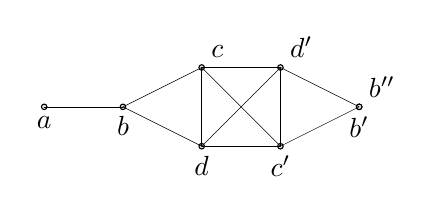
\begin{tikzpicture}
    % Definitions:
    \tkzDefPoint(0,1){a}
    \tkzDefPoint(1,1){b}
    \tkzDefPoint(2,1.5){c}
    \tkzDefPoint(2,0.5){d}
    \tkzDefPoint(3,1.5){d'}
    \tkzDefPoint(3,0.5){c'}
    \tkzDefPoint(4,1){b'}
    \tkzDefPoint(4,1){b''}
    % Drawing:
    \tkzDrawPoints(a,b,c,d,c',d',b',b'')
    \tkzDrawSegments(a,b b,c b,d c,d c,c' c,d' c,d' d,c' d,d' c',d' c',b' d',b')
    % Labels:
    \tkzLabelPoints(a,b,d,c',b')
    \tkzLabelPoints[above right](c,d',b'')
  \end{tikzpicture}

  \begin{forthel}
    \begin{theorem}[Outer Pasch] %[Gupta] % Satz 5.1
      Assume $a \neq b$.
      Assume $\Betw{a}{b}{c}$ and $\Betw{a}{b}{d}$.
      Then $\Betw{a}{c}{d}$ or $\Betw{a}{d}{c}$.
    \end{theorem}

    \begin{proof}
      Take a point $c'$ such that
        $\Betw{a}{d}{c'}$ and $\Cong{d}{c'}{c}{d}$.
      Take a point $d'$ such that
        $\Betw{a}{c}{d'}$ and $\Cong{c}{d'}{c}{d}$.
      Then $c = c'$ or $d = d'$.

      Proof.
        We have $\BetwFour{a}{b}{c}{d'}$ (by \ref{extension_to_quaternary_betweenness}).
        We have $\BetwFour{a}{b}{d}{c'}$ (by \ref{extension_to_quaternary_betweenness}).
        %
        Take a point $b'$ such that
          $\Betw{a}{c'}{b'}$ and
          $\Cong{c'}{b'}{c}{b}$ (by \ref{segment_construction}).
        Take a point $b''$ such that
          $\Betw{a}{d'}{b''}$ and
          $\Cong{d'}{b''}{b}{d}$ (by \ref{segment_construction}).
        %
        Then $\BetwFive{a}{b}{c}{d'}{b''}$.
        Then $\BetwFive{a}{b}{d}{c'}{b'}$.

        %
        Thus $\Cong{b}{c'}{b''}{c}$.

        Thus $\Cong{b}{b'}{b''}{b}$.

        We have $\Betw{a}{b}{b'}$ and $\Betw{a}{b}{b''}$.
        Thus $b'' = b'$. % (by UniqueConstruct).

        We have $\OFS{b}{c}{d'}{c'}{b'}{c'}{d}{c}$.
        Thus $\Cong{c'}{d'}{c}{d}$.

        Take a point $e$ such that
          $\Betw{c}{e}{c'}$ and $\Betw{d}{e}{d'}$.
        Then $\IFS{d}{e}{d'}{c}{d}{e}{d'}{c'}$
        and $\IFS{c}{e}{c'}{d}{c}{e}{c'}{d'}$.
        Thus $\Cong{e}{c}{e}{c'}$ and $\Cong{e}{d}{e}{d'}$.

        Case $c \neq c'$.
          We have $c\neq d'$.

          Take a point $p$ such that
            $\Betw{c'}{c}{p}$ and $\Cong{c}{p}{c}{d'}$.
          Take a point $r$ such that
            $\Betw{d'}{c}{r}$ and $\Cong{c}{r}{c}{e}$.
          Take a point $q$ such that
            $\Betw{p}{r}{q}$ and $\Cong{r}{q}{r}{p}$.

          Then $\OFS{d'}{c}{r}{p}{p}{c}{e}{d'}$.
          Thus $\Cong{r}{p}{e}{d'}$.
          Thus $\Cong{r}{q}{e}{d}$.

          Then $\OFS{d'}{e}{d}{c}{p}{r}{q}{c}$.
          Thus $\Cong{d'}{d}{p}{q}$.
          Thus $\Cong{c}{q}{c}{d}$.
          Thus $\Cong{c}{p}{c}{q}$.

          We have $\Cong{r}{p}{r}{q}$.
          We have $r \neq c$.

          Then $r$ is collinear with $c$ and $d'$.
          Thus $\Cong{d'}{p}{d'}{q}$.

          We have $c \neq d'$.
          Then $c$ is collinear with $d'$ and $b$.
          Then $c$ is collinear with $d'$ and $b'$.
          Thus $\Cong{b}{p}{b}{q}$ and $\Cong{b'}{p}{b'}{q}$.

          Thus $b \neq b'$.
          Then $b$ is collinear with $c'$ and $b'$.
          Thus $\Cong{c'}{p}{c'}{q}$.

          $c'$ is collinear with $c$ and $p$.
          Thus $\Cong{p}{p}{p}{q}$.
          Thus $p = q$.
          Thus $d = d'$.
        End.
      End.
      Therefore $\Betw{a}{c}{d}$ or $\Betw{a}{d}{c}$. %(by C5o1k).
    \end{proof}
  \end{forthel}

  \begin{forthel}
    \begin{lemma} %[D5o2]
      Assume $a \neq b$.
      If $\Betw{a}{b}{c}$ and $\Betw{a}{b}{d}$
      then $\Betw{b}{c}{d}$ or $\Betw{b}{d}{c}$.
    \end{lemma}

    \begin{theorem} %[D5o3]
      If $\Betw{x}{y}{w}$ and $\Betw{x}{z}{w}$ then $\Betw{x}{y}{z}$ or $\Betw{x}{z}{y}$.
    \end{theorem}
  \end{forthel}

  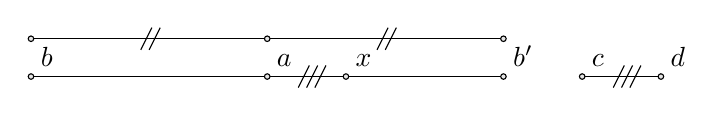
\begin{tikzpicture}
    % Points
    \tkzDefPoint(0,0.48){bv}
    \tkzDefPoint(3,0.48){av}
    \tkzDefPoint(6,0.48){bv'}
    \tkzDefPoint(0,0){b}
    \tkzDefPoint(3,0){a}
    \tkzDefPoint(4,0){x}
    \tkzDefPoint(6,0){b'}
    \tkzDefPoint(7,0){c}
    \tkzDefPoint(8,0){d}
    % Ways
    \tkzDrawSegments(b,b' c,d bv,bv')
    % Labels
    \tkzDrawPoints(b,a,b',c,d,bv,av,bv')
    \tkzDrawPoints(x)
    \tkzLabelPoints[above right](b,a,x,b',c,d)
    % Markers
    \tkzMarkSegments[mark=s||](bv,av av,bv')
    \tkzMarkSegments[mark=s|||](a,x c,d)
  \end{tikzpicture}

  \begin{forthel}
    \begin{lemma}%[ConstructOr]
      Assume $a\neq b$.
      Then
        we have $\Cong{a}{x}{c}{d}$ for some point $x$ such that
          $\Betw{a}{b}{x}$ or $\Betw{a}{x}{b}$.
        %there exist a point $x$ such that
        %($\Betw{a}{b}{x}$ or $\Betw{a}{x}{b}$) and $\Cong{a}{x}{c}{d}$.
    \end{lemma}
    \begin{proof}
      Take $b'$ such that $\Betw{b}{a}{b'}$ and $\Cong{a}{b'}{a}{b}$.
      Take $x$ such that $\Betw{b'}{a}{x}$ and $\Cong{a}{x}{c}{d}$.
    \end{proof}
  \end{forthel}

  \section{Comparing segments}

  \begin{convention}
    \begin{forthel}
      Let $a, a', b, b', c, c', d, d', e, f, x, y, z, u, v, w, p, q, r$ denote points.
    \end{forthel}
  \end{convention}

  Informally, a segment $ab$ is smaller than a segment $cd$ whenever
  we can find a subsegment $cx$
  of $cd$ of the same length as $ab$.

  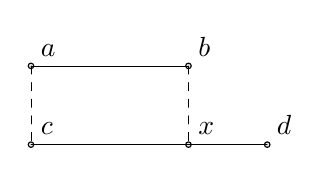
\begin{tikzpicture}
    % Points
    \tkzDefPoint(0,1){a}
    \tkzDefPoint(2,1){b}
    \tkzDefPoint(2,0){x}
    \tkzDefPoint(0,0){c}
    \tkzDefPoint(3,0){d}
    % Drawing
    \tkzDrawPoints(a,b,x,c,d)
    \tkzDrawSegments(a,b c,d)
    \tkzDrawSegments[dashed](a,c b,x)
    % Labels
    \tkzLabelPoints[above right](a,b,c,d,x)
  \end{tikzpicture}

  \begin{forthel}
    \begin{definition} % Definition 5.4 (first part)
      $\Leq{a}{b}{c}{d}$ iff there exists $x$ such that $\Betw{c}{x}{d}$ and $\Cong{a}{b}{c}{x}$.
    \end{definition}

    %\begin{definition} % Definition 5.4 (second part)
    %  $\Geq{v}{w}{p}{q}$ iff $\Leq{p}{q}{v}{w}$.
    %\end{definition}
  \end{forthel}

  Alternatively, we can say that a segment $ab$ is smaller than $cd$ whenever we can extend $ab$
  to a segment $ax$ of length $cd$.

  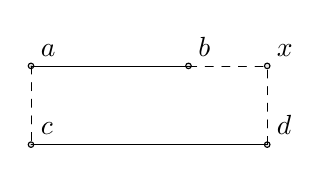
\begin{tikzpicture}
    % Points
    \tkzDefPoint(0,1){a}
    \tkzDefPoint(2,1){b}
    \tkzDefPoint(3,1){x}
    \tkzDefPoint(0,0){c}
    \tkzDefPoint(3,0){d}
    % Drawing
    \tkzDrawPoints(a,b,x,c,d)
    \tkzDrawSegments(a,b c,d)
    \tkzDrawSegments[dashed](a,c b,x d,x)
    % Labels
    \tkzLabelPoints[above right](a,b, c,d, x)
  \end{tikzpicture}

  \begin{forthel}
    \begin{lemma} % Satz 5.5 (first part)
      Assume $\Leq{a}{b}{c}{d}$.
      Then there exists $x$ such that $\Betw{a}{b}{x}$ and $\Cong{a}{x}{c}{d}$.
    \end{lemma}
    \begin{proof}
        Take $y$ such that $\Betw{c}{y}{d}$ and $\Cong{a}{b}{c}{y}$.
        Take $x$ such that $\Betw{a}{b}{x}$ and $\Cong{b}{x}{y}{d}$.
        Then $\Cong{a}{x}{c}{d}$.
    \end{proof}
  \end{forthel}

  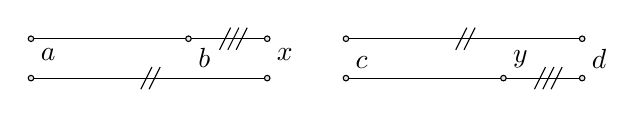
\begin{tikzpicture}
    \tkzDefPoint(0,0.5){a}
    \tkzDefPoint(3,0.5){x}
    \tkzDefPoint(0,0){av}
    \tkzDefPoint(2,0.5){b}
    \tkzDefPoint(3,0){xv}
    \tkzDefPoint(4,0){c}
    \tkzDefPoint(6,0){y}
    \tkzDefPoint(7,0){d}
    \tkzDefPoint(4,0.5){cv}
    \tkzDefPoint(7,0.5){dv}
    %
    \tkzDrawSegments(av,xv a,x cv,dv c,d)
    %
    \tkzLabelPoints[below right](a,b,x)
    \tkzLabelPoints[above right](c,y,d)
    %
    \tkzDrawPoints(av,xv,a,b,x,c,y,d,cv,dv)
    %
    \tkzMarkSegments[mark=s||](av,xv cv,dv)
    \tkzMarkSegments[mark=s|||](b,x y,d)
  \end{tikzpicture}

  \begin{forthel}
    \begin{lemma} % Satz 5.5 (second part)
      Let $x$ be a point such that $\Betw{a}{b}{x}$ and $\Cong{a}{x}{c}{d}$.
      Then $\Leq{a}{b}{c}{d}$.
    \end{lemma}
    \begin{proof}
      Take $b'$ such that $\Betw{c}{b'}{d}$ and $\SenaryCong{a}{b}{x}{c}{b'}{d}$.
    \end{proof}
  \end{forthel}



  \begin{forthel}
    \begin{lemma}[Transitivity of congruence and comparison] % Satz 5.6 (first part)
      Assume $\Cong{a}{b}{c}{d}$ and $\Leq{c}{d}{e}{f}$.
      Then $\Leq{a}{b}{e}{f}$.
    \end{lemma}
    \begin{proof}
      Take $x$ such that $\Betw{e}{x}{f}$ and $\Cong{c}{d}{e}{x}$.
    \end{proof}

    \begin{lemma}[Transitivity of comparison and congruence] % Satz 5.6 (second part)
      Assume $\Leq{a}{b}{c}{d}$ and $\Cong{c}{d}{e}{f}$.
      Then $\Leq{a}{b}{e}{f}$.
    \end{lemma}
    \begin{proof}
      Take $x$ such that $\Betw{a}{b}{x}$ and $\Cong{a}{x}{c}{d}$.
    \end{proof}

    \begin{lemma}[Reflexivity of comparison] % Satz 5.7
      For all points $a, b$ we have $\Leq{a}{b}{a}{b}$.
    \end{lemma}

    \begin{lemma}[Transitivity of comparison] % Satz 5.8
      Assume $\Leq{a}{b}{c}{d}$ and $\Leq{c}{d}{e}{f}$.
      Then $\Leq{a}{b}{c}{d}$.
    \end{lemma}
    \begin{proof}
      Take $x$ such that $\Betw{a}{b}{x}$ and $\Cong{a}{x}{c}{d}$.
      Take $y$ such that $\Betw{c}{d}{y}$ and $\Cong{c}{y}{e}{f}$.
    \end{proof}

    \begin{lemma}[Antisymmetry of comparison] % Satz 5.9
      Assume $\Leq{a}{b}{c}{d}$ and $\Leq{c}{d}{a}{b}$.
      Then $\Cong{a}{b}{c}{d}$.
    \end{lemma}
    \begin{proof}
      Take $x$ such that $\Betw{c}{x}{d}$ and $\Cong{a}{b}{c}{x}$.
      Take $y$ such that $\Betw{c}{d}{y}$ and $\Cong{a}{b}{c}{y}$.
      Then $\Cong{c}{x}{c}{y}$.
      Thus $x = d = y$.
    \end{proof}

    \begin{lemma}[Connexity of comparison] % Satz 5.10
      Let $a, b, c, d$ be points.
      Then $\Leq{a}{b}{c}{d}$ or $\Leq{c}{d}{a}{b}$.
    \end{lemma}
    \begin{proof}
      Case $a \neq b$.
        Take $x$ such that
        ($\Betw{b}{a}{x}$ or $\Betw{b}{x}{a}$) and $\Cong{b}{x}{c}{d}$.
      End.
    \end{proof}

    \begin{lemma} % Satz 5.11
      For all points $a, b, c$ we have $\Leq{a}{a}{b}{c}$.
    \end{lemma}

    \begin{lemma} % Satz 5.12 (first part)
      Assume $\Betw{a}{b}{c}$.
      Then $\Leq{a}{b}{a}{c}$.
    \end{lemma}

    \begin{lemma} % Satz 5.12 (second part)
      Assume $\Betw{a}{b}{c}$.
      Then $\Leq{b}{c}{a}{c}$.
    \end{lemma}
    \begin{proof}
      $a$ is a point such that $\Betw{c}{b}{a}$ and $\Cong{c}{a}{a}{c}$.
    \end{proof}

    \begin{lemma} % Satz 5.12 (third part)
      Assume that $a$ is collinear with $b$ and $c$.
      Assume $\Leq{a}{b}{a}{c}$ and $\Leq{b}{c}{a}{c}$.
      Then $\Betw{a}{b}{c}$.
    \end{lemma}
  \end{forthel}


  \begin{forthel}
    \begin{definition}
      $\Less{p}{q}{x}{y}$ iff $\Leq{p}{q}{x}{y}$ and $\NotCong{p}{q}{x}{y}$.
    \end{definition}

    \begin{definition}
      $\Greater{p}{q}{x}{y}$ iff $\Less{x}{y}{p}{q}$.
    \end{definition}
  \end{forthel}



  \section{Rays and lines}

  \begin{convention}
    \begin{forthel}
      Let $a, a', b, b', c, c', d, d', e, f, x, y, z, u, v, w, p, q, r$ denote points.
    \end{forthel}
  \end{convention}

  \begin{forthel}
    \begin{definition} % SST 6.1 (i)
      $a$ and $b$ lie on opposite sides of $u$ iff
      $a, b, u$ are pairwise nonequal and $\Betw{a}{u}{b}$.
    \end{definition}

    \begin{definition} % SST 6.1 (ii)
      $a$ and $b$ are equivalent with respect to $u$ iff
        $a, b\neq u$ and ($\Betw{u}{a}{b}$ or $\Betw{u}{b}{a}$).
    \end{definition}
  \end{forthel}

  \begin{convention}
    \begin{forthel}
      Let $\RelEquiv{a}{b}{u}$ stand for $a$ and $b$ are equivalent with respect to $u$.
    \end{forthel}
  \end{convention}

  We will see that two points are equivalent with respect to a point $u$
  iff they determine the same ray with origin $u$.

  \begin{forthel}
    \begin{lemma} % SST 6.2
      Suppose $a,b,c \neq u$.
      Suppose $\Betw{a}{u}{c}$.
      Then $\Betw{b}{u}{c}$ iff
        %$a$ and $b$ are equivalent with respect to $u$.
        $\RelEquiv{a}{b}{u}$.
    \end{lemma}

    \begin{lemma} % SST 6.3 (first part)
      Suppose $a$ and $b$ are equivalent with respect to $u$.
      Then $a, b\neq u$ and there exists a point $c$ such that
        $c\neq u$ and $\Betw{a}{u}{c}$ and $\Betw{b}{u}{c}$.
    \end{lemma}

    \begin{lemma} % SST 6.3 (second part)
      Suppose $a, b\neq u$.
      Suppose there exists a point $c$ such that
        $c\neq u$ and $\Betw{a}{u}{c}$ and $\Betw{b}{u}{c}$.
      Then $a$ and $b$ are equivalent with respect to $u$.
    \end{lemma}

    \begin{lemma} % SST 6.4
      $a$ and $b$ are equivalent with respect to $u$ iff
        $a$ is collinear with $u$ and $b$ and not $\Betw{a}{u}{b}$.
    \end{lemma}

    \begin{lemma}[Reflexivity of relative equivalence]
      Suppose $a\neq u$.
      Then $\RelEquiv{a}{a}{u}$.
    \end{lemma}

    \begin{lemma}[Symmetry of relative equivalence]
      If $\RelEquiv{a}{b}{u}$ then $\RelEquiv{b}{a}{u}$.
    \end{lemma}

    \begin{lemma}[Transitivity of relative equivalence]
      Assume $\RelEquiv{a}{b}{u}$ and $\RelEquiv{b}{c}{u}$.
      Then $\RelEquiv{a}{c}{u}$.
    \end{lemma}
    \begin{proof} % Giving the case distinction speeds up the proof, but E also manages without.
      Case $\Betw{u}{a}{b}$.
      End.
      %Then $\Betw{u}{b}{a}$.
    \end{proof}
  \end{forthel}

  % TODO: reasoner breaks on this definition ...
  %
  %\begin{definition} % SST 6.8 (first part)
    %  $\Ray{u}{a} = \{ \beta \mid   \RelEquiv{\beta}{a}{u} \}$.
    %\end{definition}

  % TODO this also breaks the reasoner ...
  %
  %   \begin{definition} % SST 6.8 (second part)
  %     A ray is an object $R$ such that there exist nonequal points $u,a$ such that
  %       %$R = \Ray{u}{a}$.
  %       $R = \{ \beta \mid   \RelEquiv{\beta}{a}{u} \}$.
  %   \end{definition}

  % TODO 6.9 (see how it is used first, a literal translation is a bit tedious)

  \begin{forthel}
    \begin{lemma} % SST 6.11 (existence)
      Suppose $r\neq a$ and $b\neq c$.
      Then there exists a point $x$ such that
        $\RelEquiv{x}{r}{a}$ and $\Cong{a}{x}{b}{c}$.
    \end{lemma}

    \begin{lemma} % SST 6.11 (uniqueness)
      Suppose $r\neq a$ and $b\neq c$.
      Let $x$ be a point such that
        $\RelEquiv{x}{r}{a}$ and $\Cong{a}{x}{b}{c}$.
      Let $x'$ be a point such that
        $\RelEquiv{x'}{r}{a}$ and $\Cong{a}{x'}{b}{c}$.
      Then $x' = x$.
    \end{lemma}

    \begin{lemma} % SST 6.13 (first implication)
      Suppose $\RelEquiv{a}{b}{u}$ and $\Leq{u}{a}{u}{b}$.
      Then $\Betw{u}{a}{b}$.
    \end{lemma}

    \begin{lemma} % SST 6.13 (second implication)
      Suppose $\RelEquiv{a}{b}{u}$ and $\Betw{u}{a}{b}$.
      Then $\Leq{u}{a}{u}{b}$.
    \end{lemma}
  \end{forthel}

  %\appendix
  \newpage
  \section*{Bibliography}
  \

  Michael Beeson, Julien Narboux, Freek Wiedijk (2019)
  \\ \textit{Proof-checking Euclid}
  \\ Springer, \textit{Annals of mathematics and artificial intelligence}, vol.~85, p.~213--257

  Michael Beeson, Larry Wos (2017)
  \\ \textit{Finding proofs in Tarskian geometry}
  \\ Springer, \textit{Journal of Automated Reasoning}, vol.~58, p.~181--207

  Gabriel Braun, Julien Narboux (2017)
  \\ \textit{A synthetic proof of Pappus' theorem in Tarski's geometry}
  \\ Springer, \textit{Journal of Automated Reasoning}, vol.~58, p.~209--230

  Michael Beeson (2015)
  \\ \textit{A constructive version of Tarski's geometry}
  \\ Elsevier, \textit{Annals of pure and applied logic}, vol.~166, no.~11, p.~1199--1273

  Julien Narboux (2006)
  \\ \textit{Mechanical theorem proving in Tarski's geometry}
  \\ Springer, \textit{Automated Deduction in Geometry}, p.~139--156

  Donald Ervin Knuth (1984)
  \\ \textit{Literate programming}
  \\ Oxford University Press, \textit{The Computer Journal}, vol.~27, no.~2, p.~97--111

  Wolfram Schwabhäuser, Wanda Szmielew, Alfred Tarski (1983)
  \\ \textit{Metamathematische Methoden in der Geometrie}
  \\ Springer

  Haragauri Naryan Gupta (1969)
  \\ \textit{On some axioms in the foundations of Cartesian spaces}
  % \\ Canadian Mathematical Society,
  \\ CMS,
  \textit{Canadian Mathematical Bulletin}, vol.~12, no.~6, p.~831--836

  Haragauri Naryan Gupta (1965)
  \\ \textit{An axiomatization of finite-dimensional Cartesian spaces over arbitrary ordered fields}
  \\ PAS,
  % \\ Polish Academy of Sciences,
  \textit{Bulletin of the Polish Academy of Sciences}, vol.~13, p.~550--551

  David Hilbert (1903)
  \\ \textit{Grundlagen der Geometrie}
  \\ Teubner
\end{document}
